The main goal of \rdfframes is to facilitate reasoning over the unwieldy structure of RDF graphs and expressing complex graph exploration or processing tasks using a familiar procedural API that can extract refined datasets for use in data science tasks. 

%The main goal of \rdfframes is to facilitate the use of the abundant information provided by knowledge graphs in data science tasks, such as machine learning.
%\rdfframes bridges the gap between the graph nature of knowledge graphs and the tabular format of machine learning by providing a familiar procedural API.
%This API allows for easily expressing complex graph exploration, processing or analytics tasks.

 
% \rdfframes models each complex graph traversal task as a sequence of graph operations that return an {\em RDFFrame}. 
% The main data structure in \rdfframes {\em RDFFrame} is an abstract data structure that represents the infromation extracted from the knowledge graph so far in tabular format. 
% Operators can either in the sequence of graph operations either extend the RDFframe by traversing the graph, clean and refine the RDFframe by applying a filtering, grouping, or aggregation operation on it, or join two RDFframes that are created from multiple graphs (Section~\ref{sec:data-model}).
\rdfframes extracts information from the graph through a sequence of function calls, each representing an \rdfframes operator.
The output of each operator is represented in tabular format in an abstract data structure known as an {\em RDFFrame} which represents the the information extracted so far.
\rdfframes operators can either expand the RDFFrame by by using navigational-style operators to traverse the graph, refine the RDFFrame by applying a filtering, grouping, or aggregation operation on it, or join two RDFFrames that are possibly created from multiple graphs (Section~\ref{sec:data-model}).

%The final RDFFrame is then exported in a Pandas dataframe using a special RDFFrame operator. This dataframe can be consumed by data science libraries for further analysis or visualization. 

To enable the user to perform initial exploration of RDF graphs, \rdfframes offers fundamental graph traversal functions that uncover the underlying structure of the knowledge graph. These functions return, for example, the main classes in the knowledge graph, the attributes of each class, the distribution of instances in classes, and the frequency of attributes of instances of specific classes. Guided by the initial exploration of the graph, the user can gradually build a tabular dataset (RDFFrame) through a sequence of calls to \rdfframes functions, each representing an operator. \rdfframes has an initial operator that creates the seed columns in any \rdfframe by matching a simple triple pattern ($subject$, $predicate$, $object$) to the knowledge graph triples. The initial seed columns are then creatred from the subjects, objects or predicates of the mapped triples. For example, the instances of the class "Artist" in DBpedia are the subjects of a ($actor$, $rdf$:$type$, $dbpo$:$Actor$) pattern. The films and their star actors are the subjects and objects of the pattern ($film$, $dbo$:$starring$, $actor$) respectively. To add more columns, \rdfframes expands the existing columns by navigating through the graph edges (i.e., RDF predicates) starting from the entities in one column to reach target entities that will be added as a new column in the \rdfframe. For example, to get the origin country of each actor, the actor coulmn is expanded following the $dbo$:$birthPlace$ predicate.
%Some \rdfframes operators are navigational, creating a column with all entities that satisfy some condition (e.g., all entities that belong to a certain class), or navigating through RDF predicates (i.e., graph edges) from the entities in one column to reach target entities that are added as a new column.
The user can also apply operations on the RDFFrame like filtering, grouping, aggregation, filtering based on aggregation values, sorting, and %finally
choosing the columns to be projected in the final RDFFrame. All these operators are relational operators that are called on an abstract relational table (e.i. \rdfframe) that hides the complexity of implementing it on the knowledge graph (e.g., using \sparql patterns).
%%the syntax and semantics of the internal graph patterns (e.g. \sparql patterns) used to implement them.
The final RDFFrame is then exported in a pandas dataframe that can be consumed by data science libraries for further analysis or visualization. 


\begin{figure}
	\centering
	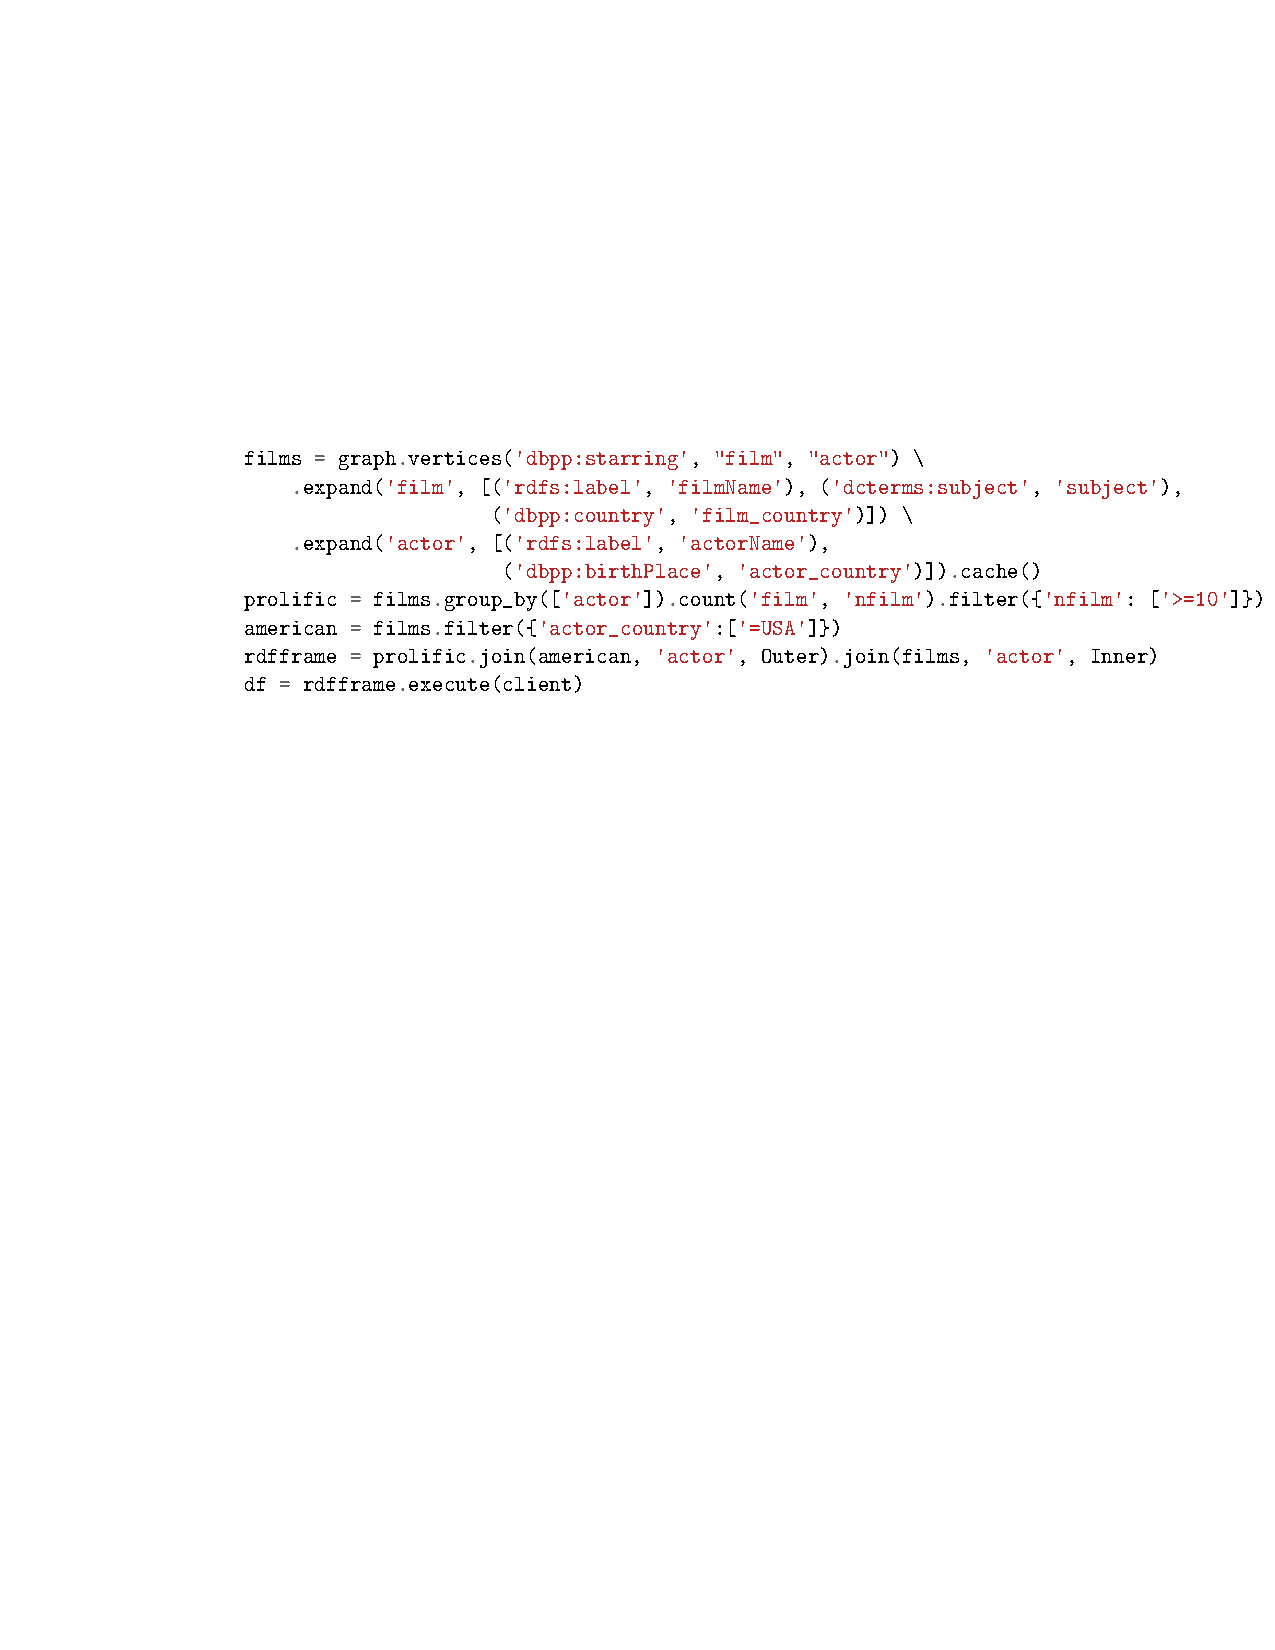
\includegraphics[width=1.0 \columnwidth]{figures/rdfframes_overview.pdf}
	\caption{\rdfframes code to extract films starred by American or prolific actors from DBpedia. \texttt{vertices('dbpp:starring')} returns the subjects and objects of \texttt{(?film, dbpp:starring, ?actor)} triples.}
	\label{fig:rdfframes}
\end{figure}


Figure~\ref{fig:rdfframes} shows an example of \rdfframes Python code that constructs a dataframe of films starred by American or prolific actors who starred in more than 10 films from DBPedia knowledge graph. 
This code returns an RDFFrame having as columns these films and their attributes (e.g., film name, actor, film country, actor country, and film topic). 
A \sparql query written by an expert to return the same result is shown in Listing~\ref{lst:overview_query}. 
We posit that many data scientists would prefer composing the few lines of Python calls and getting the result already structured in a dataframe than composing this \sparql query.
%The figure shows that a complex data retrieval task such as this can be expressed in a few lines of Python, using a navigational-style API that would be familiar to data scientists and easily intergated with the PyData stack. 
%Note that the \sparql query is non-trivial, and we posit that many data scientists would prefer composing the API calls and getting the result already structured in a DataFrame as in Figure ~\ref{fig:topic_modelling} to composing this query.

\begin{lstlisting}[
language=SQL,
showspaces=false,
basicstyle=\ttfamily\scriptsize,
commentstyle=\color{gray},
caption={SPARQL query corresponding to \rdfframes code shown in Figure~\ref{fig:rdfframes}.},
label={lst:overview_query}
]

SELECT  ?actorName ?filmName ?subject ?film_country ?actor_country
FROM <http://dbpedia.org>
WHERE
  {   { ?film   dbpprop:starring    ?actor ;
                rdfs:label          ?filmName ;
                dcterms:subject     ?subject ;
                dbpprop:country     ?film_country .
        ?actor  rdfs:label          ?actorName ;
                dbpprop:birthPlace  ?actor_country
        FILTER ( langMatches(lang(?actorName), "en") && ( ?actor_country = "USA" ) )
      }
    UNION
      { SELECT  ?actorName ?filmName ?subject ?film_country ?actor_country
        WHERE
          { ?film   dbpprop:starring    ?actor ;
                    rdfs:label          ?filmName ;
                    dcterms:subject     ?subject ;
                    dbpprop:country     ?film_country .
            ?actor  rdfs:label          ?actorName ;
                    dbpprop:birthPlace  ?actor_country
            { SELECT  ?actor
              WHERE
                { ?film  dbpprop:starring  ?actor }
              GROUP BY ?actor
              HAVING ( ( COUNT(DISTINCT ?film) >= 10 ) && ( COUNT(DISTINCT ?film) <= 20 ) )
            }
          }
      }
  }
\end{lstlisting}

\begin{figure}
	\centering
	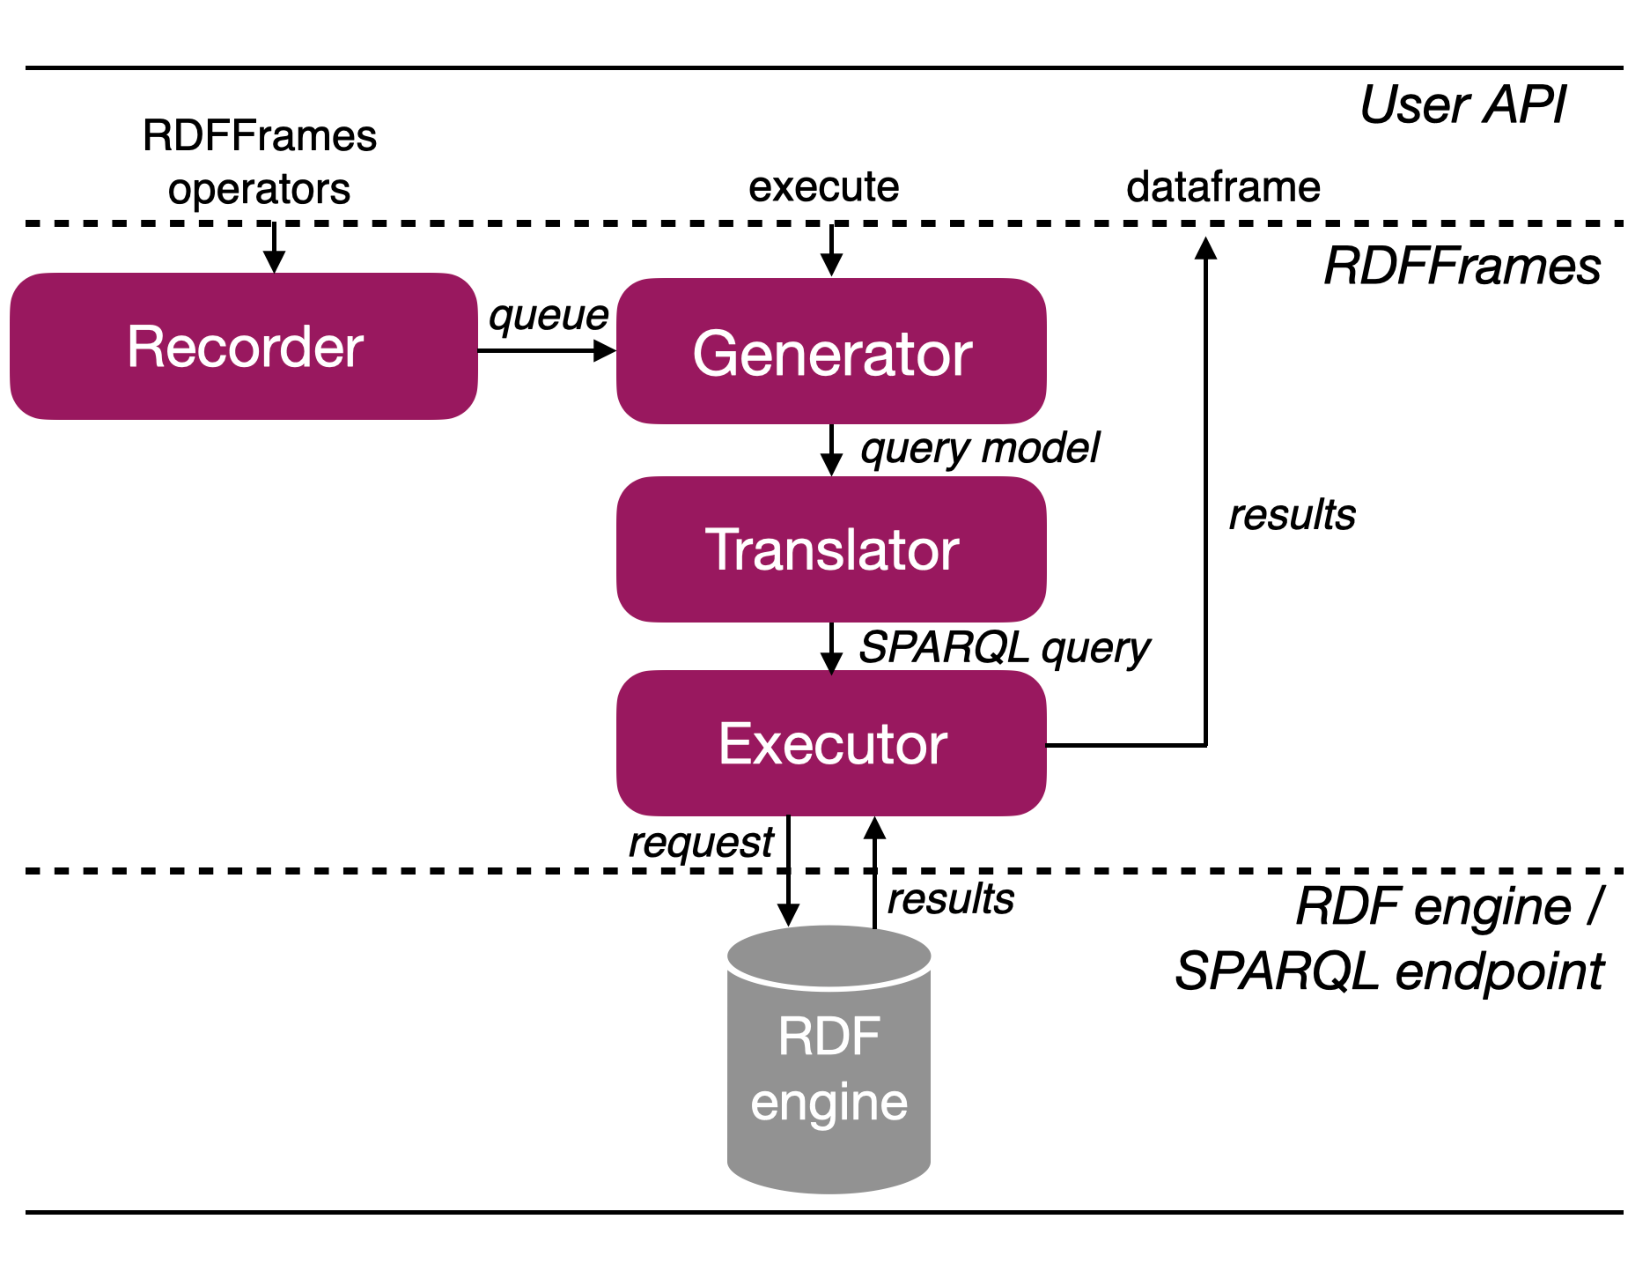
\includegraphics[width=0.8 \columnwidth]{figures/architecture}
	\caption{\rdfframes architecture.}
	\label{fig:architecture}
\end{figure}

% starting by one of the fundamental functions offerred by the API or by traversing the knowledge graph starting from a specific node (representing a class or instance) or edge (representiung an attribute) and retrieving all the nodes connected to it. This initial RDFframe is then expanded by further traversal of the graph or by joining it with other RDFframes. The user can aslo apply more complex operations on it like filtering, grouping, aggregation, filters based on aggregations,  sorting and finally choosing the columns to be projected in the final RDFFrame. All these operators are relational operators called on an abstract relational table that hides the complexity of the syntax and semantics of the internal graph patterns (e.g. \sparql patterns) used to implement them. The final RDFframe is then exported in a dataframe that can be fed to the data sceince libraries for further analysis or visualization. 

Internally, \rdfframes  converts the sequence of operators called by the user to a compact SPARQL query, execute this query on an RDF engine or SPARQL endpoint, and returns the results in a dataframe. Figure~\ref{fig:architecture} shows the components of \rdfframes architecture that implements these steps. First, \rdfframes records the operators invoked by the user without executing them as it follows a lazy evaluation strategy and. The \texttt{Recorder} stores in a queue the sequence of operators by keeping one FIFO queue per RDFFrame. % so that it maintains a deterministic behavior described by an ordered sequence of operators. 
The end of the sequence of calls is markd by the special \rdfframes \texttt{execute} operator which requests the materialization of the final RDFFrame. 
%\rdfframes avoids the construction and execution of partial \sparql queries which would then require external join operations in Python.
At this point, the \texttt{Generator} consumes the operators in the queue to build a {\em query model} representing the user's code (Section~\ref{sec:query-generation}).
The query model is an intermediate representation that resembles a \sparql query. The goal of the query model is (i)~to separate the API parsing logic from the query building logic for flexible manipulation and implementation, and (ii)~to facilitate optimization techniques for building the queries, especially in the case of nested queries. Next, the \texttt{Translator} translates the query model into a \sparql query. This process includes validating the query model to ensure a valid \sparql syntax and its equivalence with the user's calls. Finally, the \texttt{Executor} sends the generated \sparql query to an RDF engine or SPARQL endpoint, handles the communication between the client and the RDF engine/endpoint, and returns the results to the user in a dataframe. The dataframe that \rdfframes returns is semantically equivalent with the results set of the generated \sparql query (Section~\ref{sec:correctness}). \rdfframes constructs as few \sparql queries as possible in order to push all the computation down to an optimized RDF engine and leverage its efficiency. Thus, lazy evaluation is crucial for optimizing execution time in \rdfframes. 


%\rdfframes follows a lazy evaluation strategy as it records the API calls made by the user. The call to the \texttt{execute} function marks the end of the sequence of calls made by the user. \rdfframes translates this sequence of operators to a \sparql query, sends it to an \sparql endpoint and returns the result in a dataframe. 
%Figure~\ref{fig:architecture} shows the components of \rdfframes architecture. At the top of the figure is the interface exposed to the user. \rdfframes exposes all operators to the user as functions that return an RDFFrame. 
%The \texttt{Recorder} stores in a queue the sequence of operators that the user invokes on an RDFFrame. \rdfframes keeps one queue per RDFFrame so that it maintains a deterministic behavior described by an ordered sequence of operators. 
%A user invokes the \texttt{execute} function on RDFFrame $D$ to signal the end of the sequence of operators and request the materialization of the final RDFFrame described by the operations called so far on $D$.
%At this point, the \texttt{Generator} consumes the operators in the queue in the order they were added to build a {\em query model} representing the user's code
%(Section~\ref{sec:query-generation}).
%The query model is an intermediate representation that resembles a \sparql query. The goal of the query model is (i)~to separate the API parsing logic from the query building logic for flexible manipulation and implementation, and (ii)~to facilitate optimization techniques for building the queries, especially in the case of nested queries. Next, the \texttt{Translator} translates the query model into a \sparql query. This process includes validating the query model to ensure a valid \sparql syntax and its equivalence with the user's calls. Finally, the \texttt{Executor} sends the generated \sparql query to an RDF engine or SPARQL endpoint, handles the communication between the client and the RDF engine/endpoint, and returns the results to the user in a dataframe. The dataframe that \rdfframes returns is semantically equivalent with the results set of the generated \sparql patterns (Section~\ref{sec:correctness}).






\iffalse
\begin{lstlisting}[
language=Python,
keywordstyle=\bfseries,
showspaces=false,
basicstyle=\ttfamily\scriptsize,
otherkeywords={expand, filter, group_by, join, edge_subs_objs, .count},
keywordstyle=\color{deepblue},
commentstyle=\color{gray},
caption={\rdfframes code to extract american actors and prolific actors.},
label={lst:overview_python}
]
films = graph.edge_subs_objs("dbpp:starring","film", "actor") \
    .expand("actor",[("dbpp:birthPlace","actor_country")])
prolific_actors = films.group_by(["actor"]) \
.count("film", "film_count") \
.filter({"film_count": ">=10"})
american_actors = films.filter({"actor_country": "=USA"})
joined_dataset = prolific_actors.join(american_actors, "actor", OuterJoin) \
.expand("film", [("rdfs:label", "filmName"), ("dcterms:subject", "subject"), ("dbpp:country", "film_country")])
.expand("actor",[("rdfs:label", "actorName"), ("dbpp:birthPlace", "actor_country")])
\end{lstlisting}
\fi
